\subsubsection{Gripper}

\begin{enumerate}
  \item 
	\textbf{Module tasks:}
	  this module should collect game elements which lies in front of the robot into the box in the back side of the robot and also it prevents to fall out game elements while driving.
  \item 
	\textbf{Construction:} 
	  module presents as two axes which connected with a chain and also inclined plane. %(figure \ref{Gripper500}).
	  %\begin{figure}[H]
	  %	\begin{minipage}[h]{1\linewidth}
	  %		\center{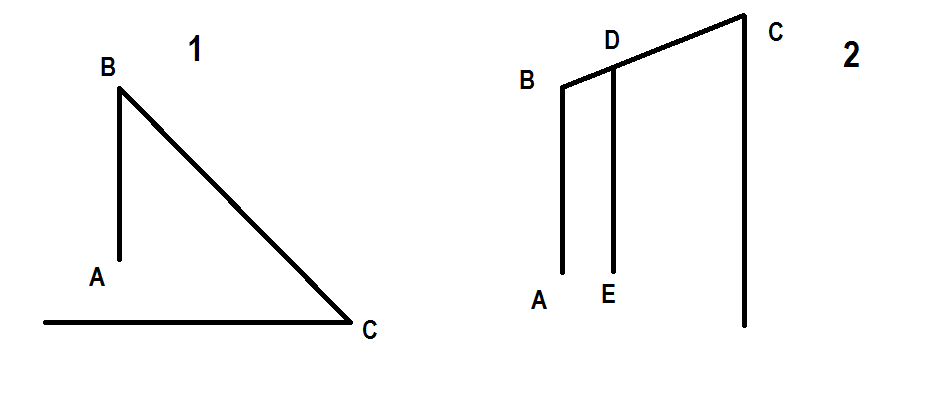
\includegraphics[scale=0.2]{3Engineering/6Specifications_for_modules/gripper/images/01}}
	  %		\caption{Gripper falities}
	  %		\label{Gripper500}
	  %	\end{minipage}
	  %\end{figure}
	  
	  There are DC motor which connected to axis with step-up gear 1/2 for speed increase, this axis located in the middle of the robot. Second axis which located in the forward side 
	  of the robot driven with chainsaw and gearing for synchronises movement with first axis. For collecting game elements there are rubber pipes 0.5cm diameter and 16cm length all 
	  along axes for game elements collecting. Axes presents as hollow metal pipes 1.5cm diameter with apertures for the screws which fix rubber pipes (figure \ref{Gripper600}).
      \begin{figure}[H]
      	\begin{minipage}[h]{1\linewidth}
      		\center{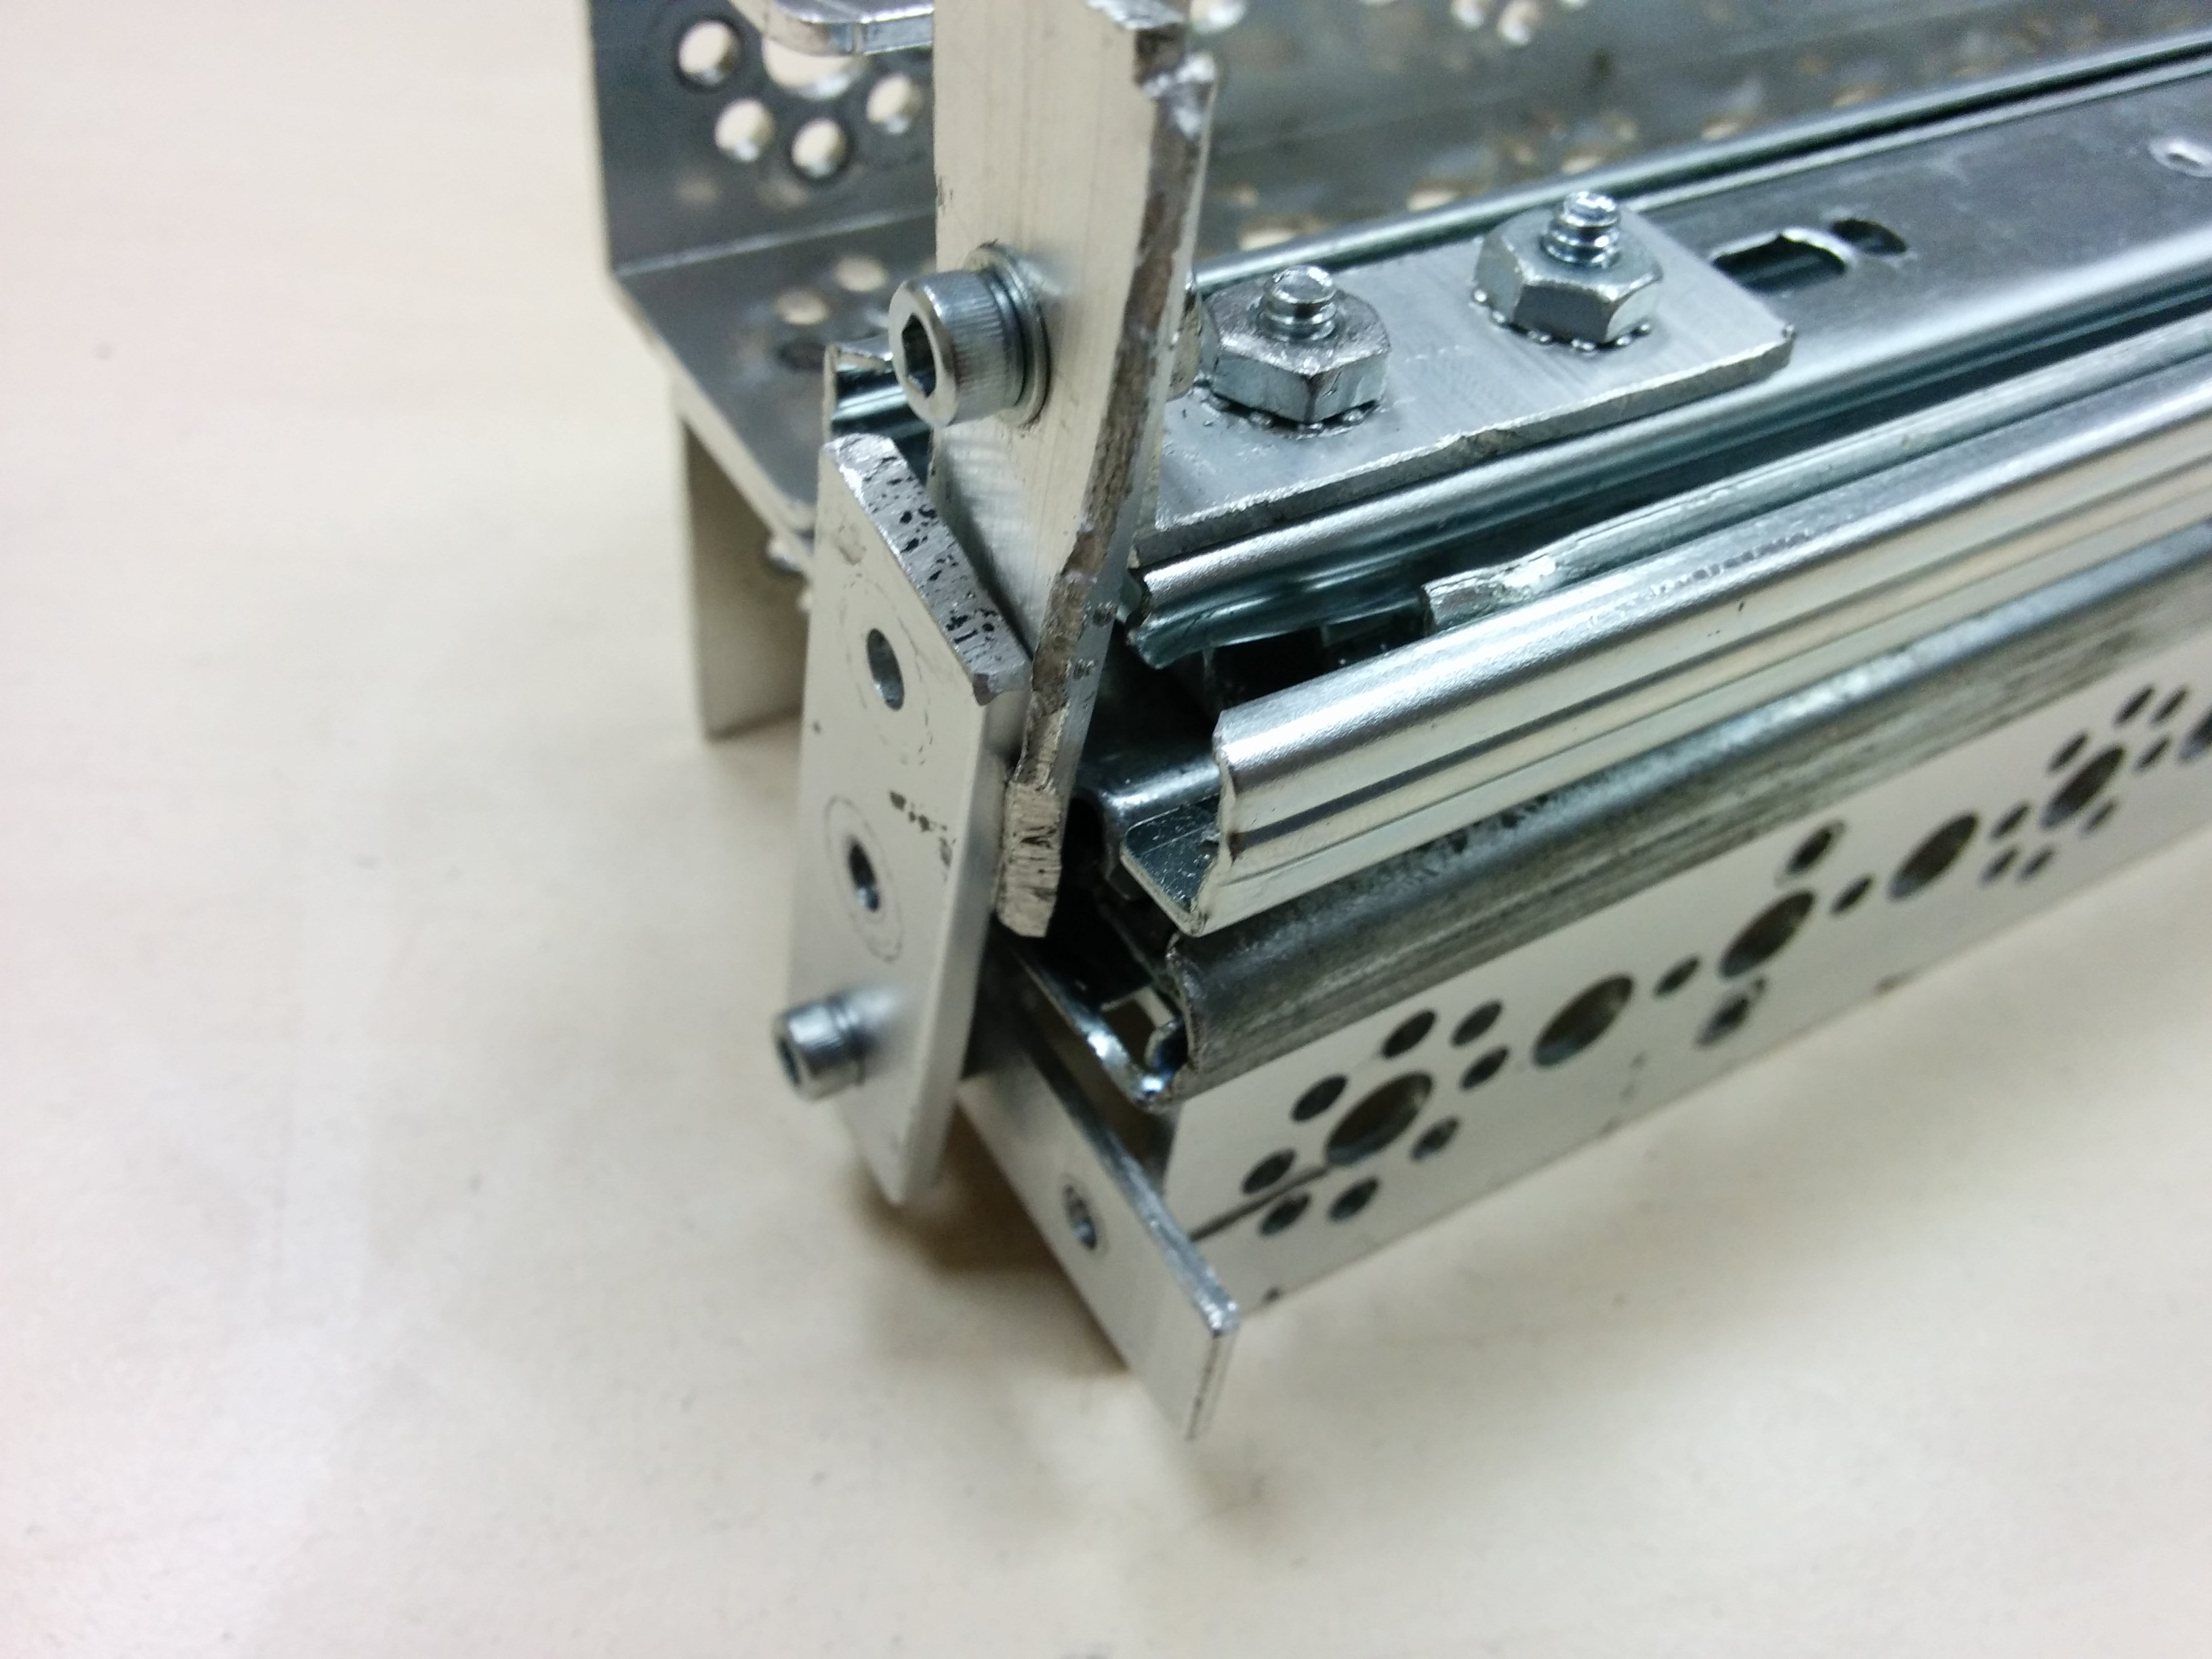
\includegraphics[scale=0.2]{3Engineering/6Specifications_for_modules/gripper/images/02}}
      		\caption{Blades on a axis}
      		\label{Gripper600}
      	\end{minipage}
      \end{figure}
      
	  Inclined plane uses to uplift game elements to the box and slopes serve as protection against game elements ingress in other parts of the robot and to direct game elements into 
	  box (figure \ref{Gripper700}).
      \begin{figure}[H]
      	\begin{minipage}[h]{1\linewidth}
      		\center{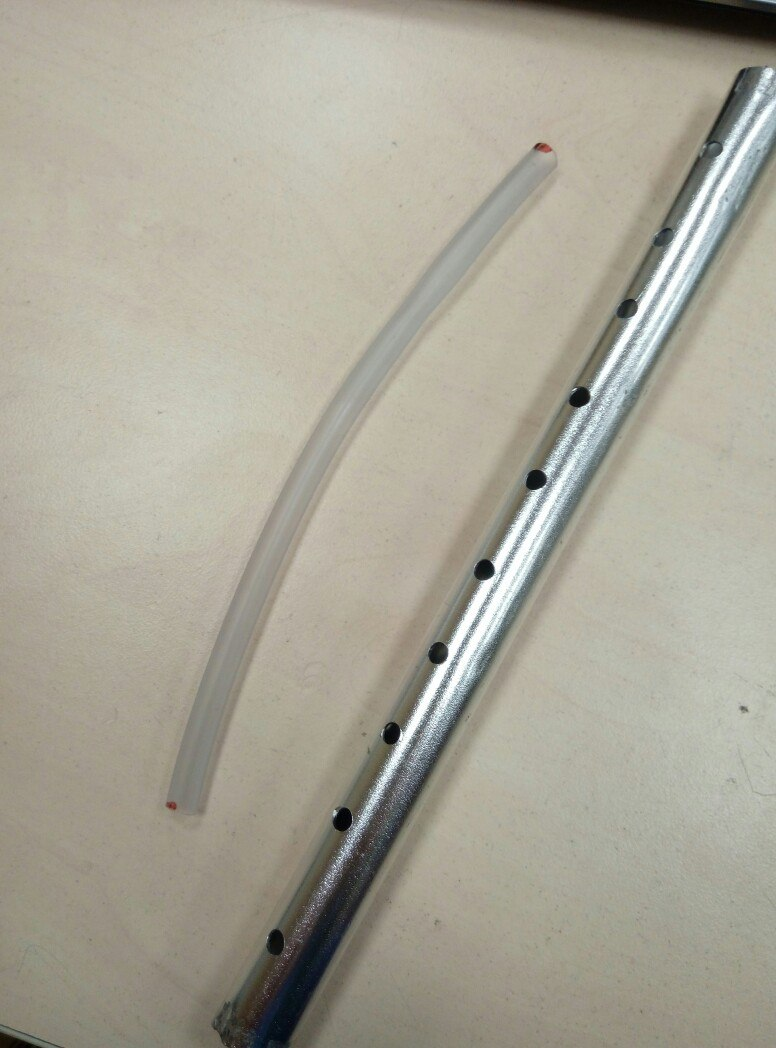
\includegraphics[scale=0.2]{3Engineering/6Specifications_for_modules/gripper/images/03}}
      		\caption{Side view of beams onto which the bucket is mounted}
      		\label{Gripper700}
      	\end{minipage}
      \end{figure}
      
      Inclined plane made from aluminium plates, slopes made from aluminium and plastic. For calculations of angles, lengths had been used GeoGebra. %(figure \ref{Gripper800}).
      %\begin{figure}[H]
      %	\begin{minipage}[h]{1\linewidth}
      %		\center{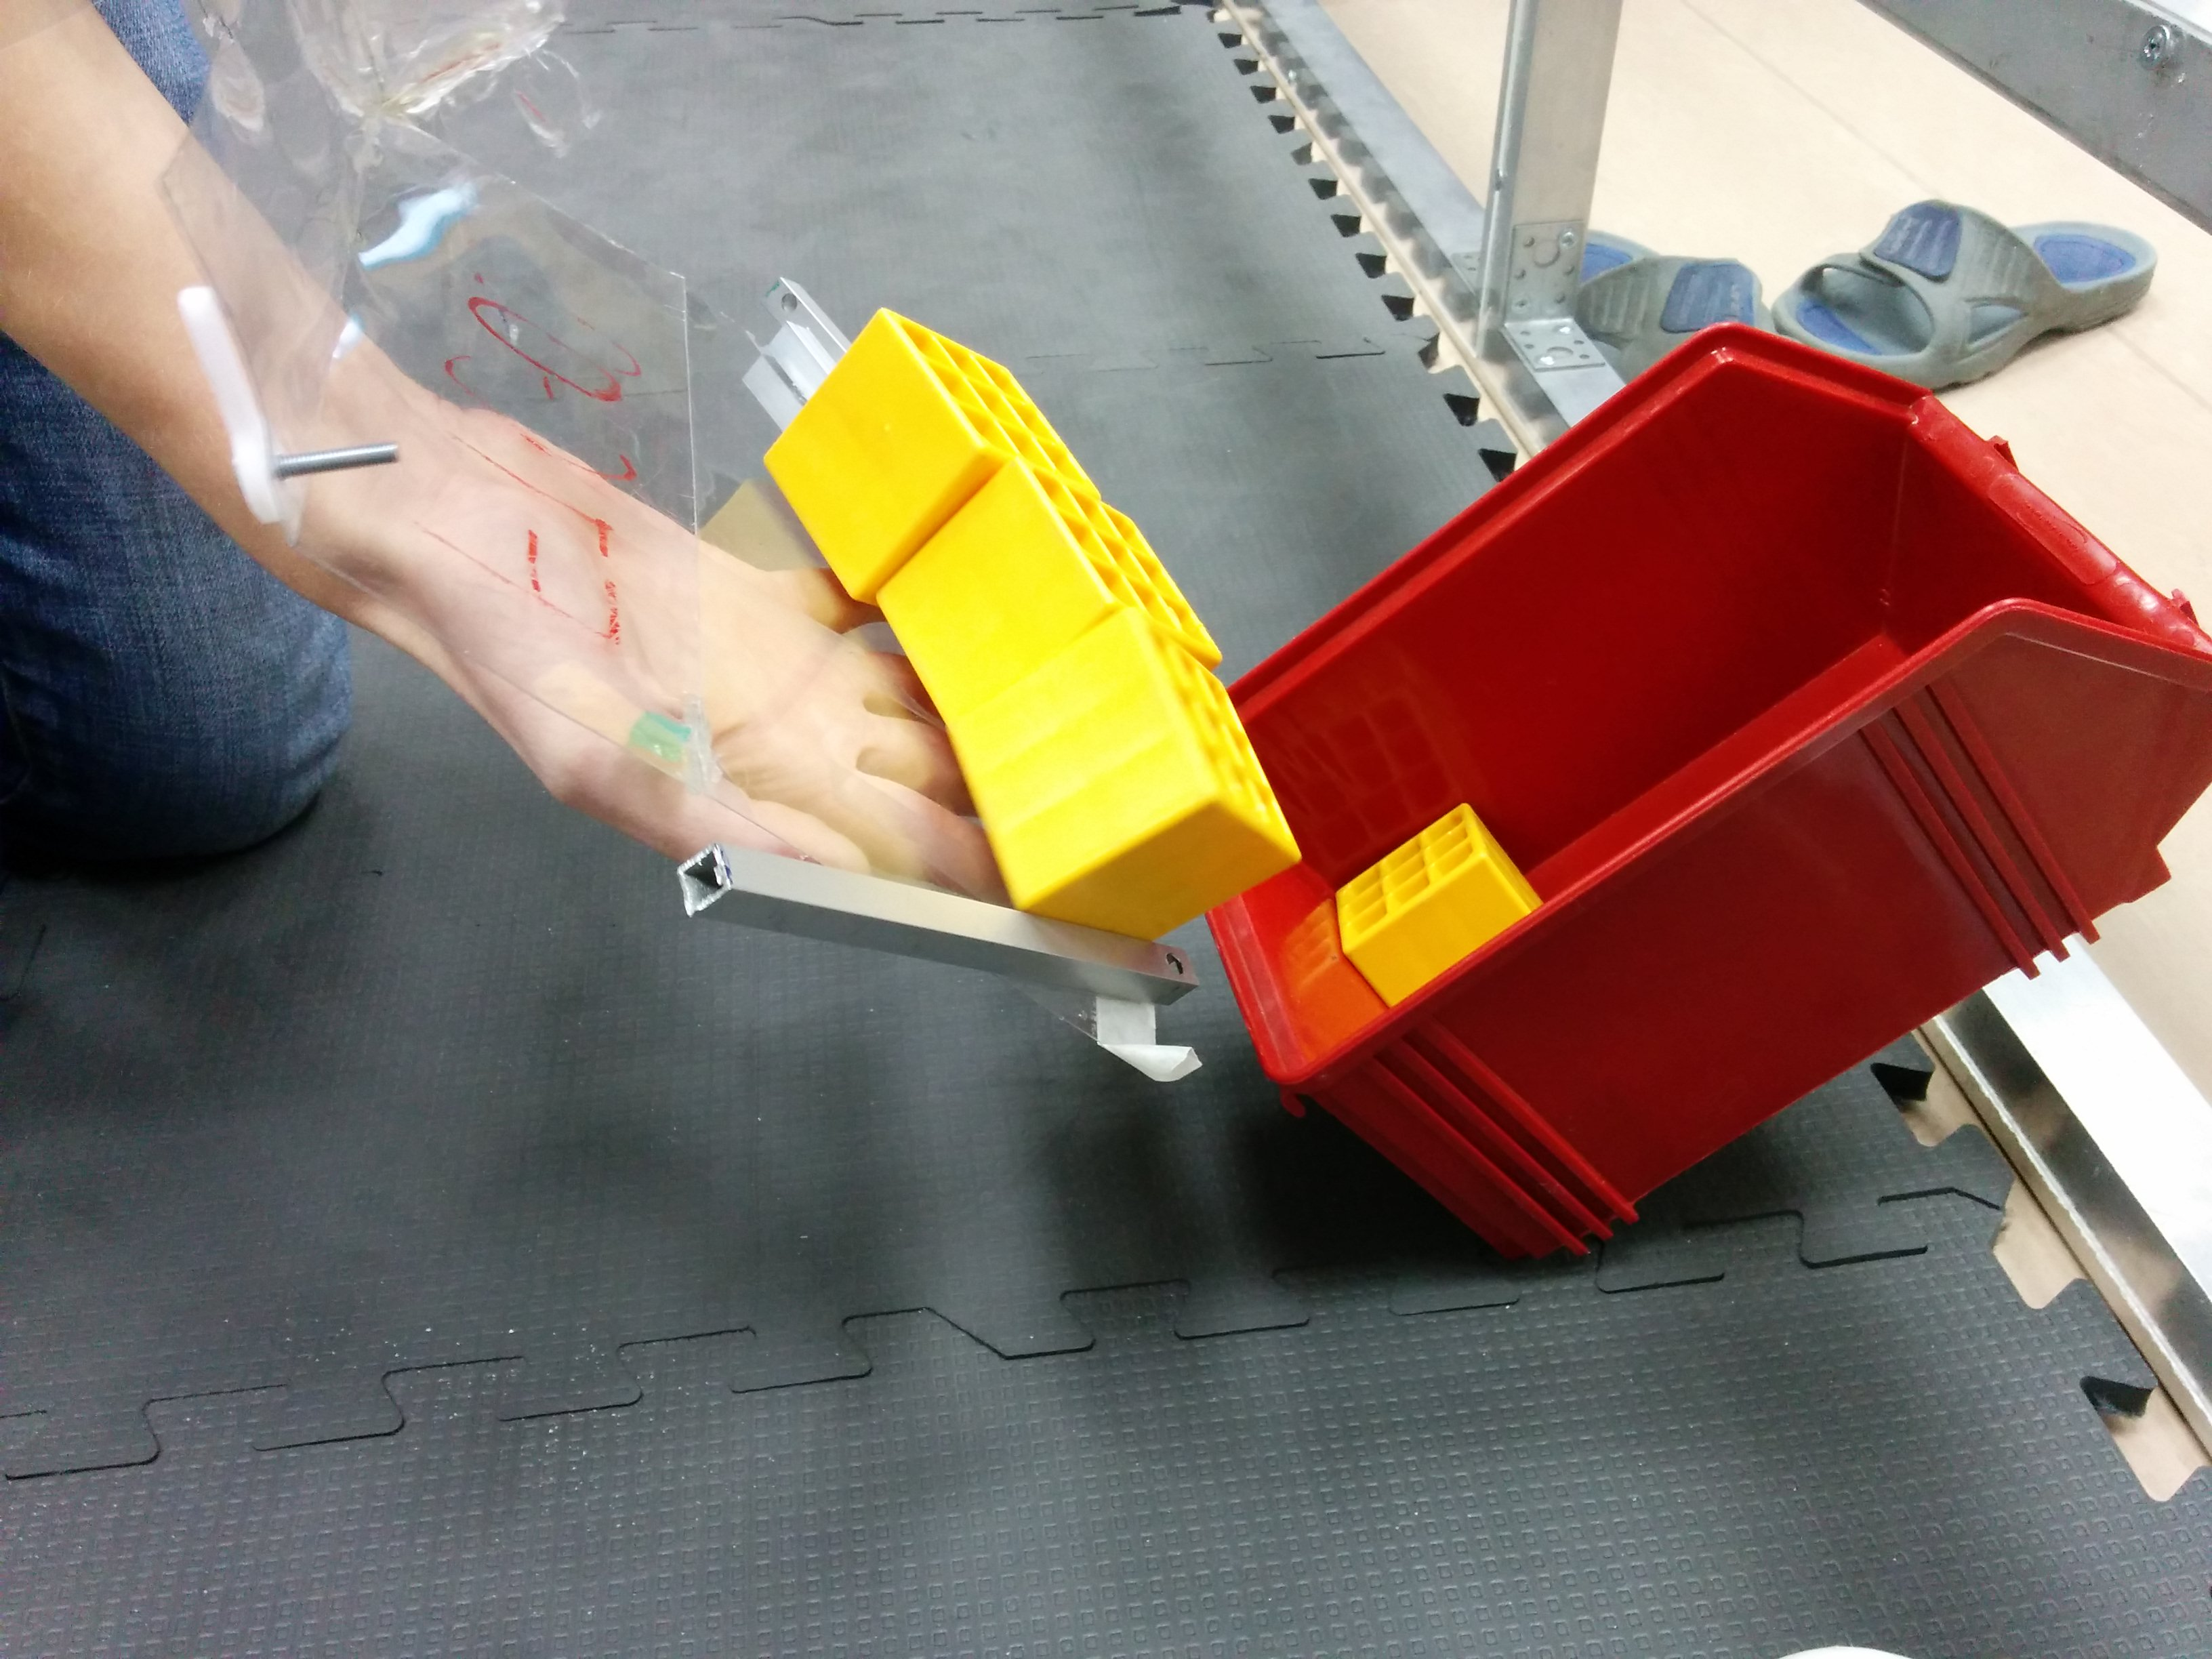
\includegraphics[scale=0.2]{3Engineering/6Specifications_for_modules/gripper/images/04}}
      %		\caption{GeoGeabra workspace with open scheme оf gripper}
      %		\label{Gripper800}
      %	\end{minipage}
      %\end{figure}
      
  \item
    \textbf{Stages of realization}
      in first version had been used two continuous rotation servos fixed on both edges of axis instead of on one DC motors but after tests this construction was rejected because of lack 
      of speed and power. Also in first version was only one forward axis but second one had been added because of box had been replaced in the backward side of the robot and higher that 
      it was in the beginning  
\end{enumerate}

\fillpage